The values $\lambda\in\left\{ 0,10^{-8},10^{-6},10^{-4},10^{-2},1\right\} $
were chosen for the ridge regression task. Figure \ref{fig:ridge-regression}
shows the corresponding plots. The lowest $\mathcal{L}^{2}$ error
norm is achieved for $\lambda=10^{-6}$. Therefore, if the examples are assumed to be uniformly distributed on $[0,1]$, the best generalization (with respect to squared-error loss function) is achieved for $\lambda=10^{-6}$.

\begin{figure}
\centering{}% This file was created by matplotlib v0.1.0.
% Copyright (c) 2010--2014, Nico Schlömer <nico.schloemer@gmail.com>
% All rights reserved.
% 
% The lastest updates can be retrieved from
% 
% https://github.com/nschloe/matplotlib2tikz
% 
% where you can also submit bug reports and leavecomments.
% 
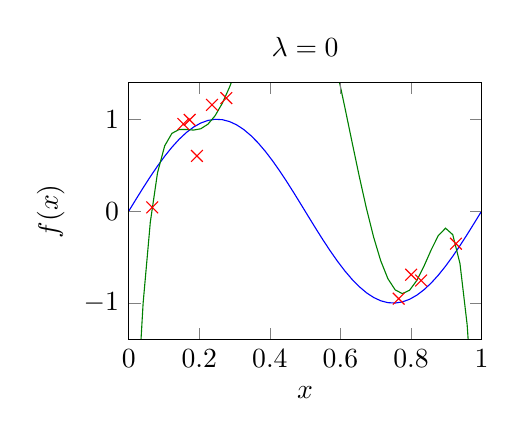
\begin{tikzpicture}

\begin{axis}[
title={$\lambda =0$},
xlabel={$x$},
ylabel={$f(x)$},
xmin=0, xmax=1,
ymin=-1.4, ymax=1.4,
axis on top,
width=0.5\textwidth,
height=0.4\textwidth
]
\addplot [red, mark=x, mark size=3, only marks]
coordinates {
(0.236048089737435,1.15627363601475)
(0.15497227080241,0.948250349180675)
(0.0665150956795899,0.0414178360950077)
(0.800452351495809,-0.690913425000795)
(0.765162602505438,-0.951934188124491)
(0.27668264344145,1.23021694041087)
(0.172664529285369,0.993397777097462)
(0.92747563142806,-0.354104773238093)
(0.828920048778419,-0.754422446814427)
(0.19343561801924,0.600940658157845)

};
\addplot [blue]
coordinates {
(0,0)
(0.0204081632653061,0.127877161684506)
(0.0408163265306122,0.253654583909507)
(0.0612244897959184,0.375267004879374)
(0.0816326530612245,0.490717552003938)
(0.102040816326531,0.598110530491216)
(0.122448979591837,0.695682550603486)
(0.142857142857143,0.78183148246803)
(0.163265306122449,0.855142763005346)
(0.183673469387755,0.914412623015812)
(0.204081632653061,0.95866785303666)
(0.224489795918367,0.98718178341445)
(0.244897959183673,0.999486216200688)
(0.26530612244898,0.995379112949198)
(0.285714285714286,0.974927912181824)
(0.306122448979592,0.93846842204976)
(0.326530612244898,0.886599306373)
(0.346938775510204,0.820172254596956)
(0.36734693877551,0.740277997075316)
(0.387755102040816,0.648228395307788)
(0.408163265306122,0.545534901210549)
(0.428571428571429,0.433883739117558)
(0.448979591836735,0.315108218023621)
(0.469387755102041,0.191158628701373)
(0.489795918367347,0.0640702199807132)
(0.510204081632653,-0.064070219980713)
(0.530612244897959,-0.191158628701372)
(0.551020408163265,-0.31510821802362)
(0.571428571428571,-0.433883739117558)
(0.591836734693878,-0.545534901210548)
(0.612244897959184,-0.648228395307788)
(0.63265306122449,-0.740277997075315)
(0.653061224489796,-0.820172254596956)
(0.673469387755102,-0.886599306373)
(0.693877551020408,-0.93846842204976)
(0.714285714285714,-0.974927912181823)
(0.73469387755102,-0.995379112949198)
(0.755102040816326,-0.999486216200688)
(0.775510204081633,-0.98718178341445)
(0.795918367346939,-0.958667853036661)
(0.816326530612245,-0.914412623015813)
(0.836734693877551,-0.855142763005346)
(0.857142857142857,-0.78183148246803)
(0.877551020408163,-0.695682550603487)
(0.897959183673469,-0.598110530491217)
(0.918367346938775,-0.490717552003939)
(0.938775510204082,-0.375267004879375)
(0.959183673469388,-0.253654583909507)
(0.979591836734694,-0.127877161684507)
(1,-2.44929359829471e-16)

};
\addplot [green!50.0!black]
coordinates {
(0,-4.33325288661144)
(0.0204081632653061,-2.35684440907392)
(0.0408163265306122,-1.00222865794249)
(0.0612244897959184,-0.119306433316764)
(0.0816326530612245,0.417474992912126)
(0.102040816326531,0.711552895156767)
(0.122448979591837,0.846568141272845)
(0.142857142857143,0.888572268742496)
(0.163265306122449,0.888122589901724)
(0.183673469387755,0.882265326211813)
(0.204081632653061,0.89640677157485)
(0.224489795918367,0.946072484693161)
(0.244897959183673,1.03855451047288)
(0.26530612244898,1.17444663047151)
(0.285714285714286,1.34906764238954)
(0.306122448979592,1.55377266860601)
(0.326530612244898,1.7771524937583)
(0.346938775510204,2.00612093136556)
(0.36734693877551,2.22689021949687)
(0.387755102040816,2.42583444548261)
(0.408163265306122,2.59024099967037)
(0.428571428571429,2.70895005822483)
(0.448979591836735,2.7728820949716)
(0.469387755102041,2.77545342228506)
(0.489795918367347,2.71287976102025)
(0.510204081632653,2.58436783948922)
(0.530612244897959,2.39219502148)
(0.551020408163265,2.14167696332209)
(0.571428571428571,1.84102329999315)
(0.591836734693878,1.5010813602717)
(0.612244897959184,1.13496791093364)
(0.63265306122449,0.757588929991357)
(0.653061224489796,0.385047408978949)
(0.673469387755102,0.0339391842794043)
(0.693877551020408,-0.279463202502228)
(0.714285714285714,-0.540138615122657)
(0.73469387755102,-0.735357404240631)
(0.755102040816326,-0.855833459911878)
(0.775510204081633,-0.896988235042158)
(0.795918367346939,-0.860326739792981)
(0.816326530612245,-0.754925506945256)
(0.836734693877551,-0.599032528222096)
(0.857142857142857,-0.421779161559698)
(0.877551020408163,-0.265004009341055)
(0.897959183673469,-0.185188767582758)
(0.918367346938775,-0.255506046082019)
(0.938775510204082,-0.567979159508241)
(0.959183673469388,-1.23575388946779)
(0.979591836734694,-2.39548221750692)
(1,-4.20981802908272)

};
\path [draw=black, fill opacity=0] (axis cs:13,1.4)--(axis cs:13,1.4);

\path [draw=black, fill opacity=0] (axis cs:1,13)--(axis cs:1,13);

\path [draw=black, fill opacity=0] (axis cs:13,-1.4)--(axis cs:13,-1.4);

\path [draw=black, fill opacity=0] (axis cs:0,13)--(axis cs:0,13);

\end{axis}

\end{tikzpicture}\hfill{}% This file was created by matplotlib v0.1.0.
% Copyright (c) 2010--2014, Nico Schlömer <nico.schloemer@gmail.com>
% All rights reserved.
% 
% The lastest updates can be retrieved from
% 
% https://github.com/nschloe/matplotlib2tikz
% 
% where you can also submit bug reports and leavecomments.
% 
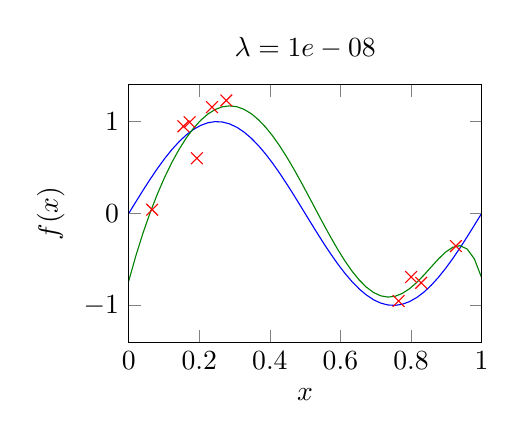
\begin{tikzpicture}

\begin{axis}[
title={$\lambda =1e-08$},
xlabel={$x$},
ylabel={$f(x)$},
xmin=0, xmax=1,
ymin=-1.4, ymax=1.4,
axis on top,
width=0.5\textwidth,
height=0.4\textwidth
]
\addplot [red, mark=x, mark size=3, only marks]
coordinates {
(0.236048089737435,1.15627363601475)
(0.15497227080241,0.948250349180675)
(0.0665150956795899,0.0414178360950077)
(0.800452351495809,-0.690913425000795)
(0.765162602505438,-0.951934188124491)
(0.27668264344145,1.23021694041087)
(0.172664529285369,0.993397777097462)
(0.92747563142806,-0.354104773238093)
(0.828920048778419,-0.754422446814427)
(0.19343561801924,0.600940658157845)

};
\addplot [blue]
coordinates {
(0,0)
(0.0204081632653061,0.127877161684506)
(0.0408163265306122,0.253654583909507)
(0.0612244897959184,0.375267004879374)
(0.0816326530612245,0.490717552003938)
(0.102040816326531,0.598110530491216)
(0.122448979591837,0.695682550603486)
(0.142857142857143,0.78183148246803)
(0.163265306122449,0.855142763005346)
(0.183673469387755,0.914412623015812)
(0.204081632653061,0.95866785303666)
(0.224489795918367,0.98718178341445)
(0.244897959183673,0.999486216200688)
(0.26530612244898,0.995379112949198)
(0.285714285714286,0.974927912181824)
(0.306122448979592,0.93846842204976)
(0.326530612244898,0.886599306373)
(0.346938775510204,0.820172254596956)
(0.36734693877551,0.740277997075316)
(0.387755102040816,0.648228395307788)
(0.408163265306122,0.545534901210549)
(0.428571428571429,0.433883739117558)
(0.448979591836735,0.315108218023621)
(0.469387755102041,0.191158628701373)
(0.489795918367347,0.0640702199807132)
(0.510204081632653,-0.064070219980713)
(0.530612244897959,-0.191158628701372)
(0.551020408163265,-0.31510821802362)
(0.571428571428571,-0.433883739117558)
(0.591836734693878,-0.545534901210548)
(0.612244897959184,-0.648228395307788)
(0.63265306122449,-0.740277997075315)
(0.653061224489796,-0.820172254596956)
(0.673469387755102,-0.886599306373)
(0.693877551020408,-0.93846842204976)
(0.714285714285714,-0.974927912181823)
(0.73469387755102,-0.995379112949198)
(0.755102040816326,-0.999486216200688)
(0.775510204081633,-0.98718178341445)
(0.795918367346939,-0.958667853036661)
(0.816326530612245,-0.914412623015813)
(0.836734693877551,-0.855142763005346)
(0.857142857142857,-0.78183148246803)
(0.877551020408163,-0.695682550603487)
(0.897959183673469,-0.598110530491217)
(0.918367346938775,-0.490717552003939)
(0.938775510204082,-0.375267004879375)
(0.959183673469388,-0.253654583909507)
(0.979591836734694,-0.127877161684507)
(1,-2.44929359829471e-16)

};
\addplot [green!50.0!black]
coordinates {
(0,-0.73515028577362)
(0.0204081632653061,-0.45794741226615)
(0.0408163265306122,-0.209298813840461)
(0.0612244897959184,0.0142431710734962)
(0.0816326530612245,0.215250654715764)
(0.102040816326531,0.395554969033175)
(0.122448979591837,0.556373213452874)
(0.142857142857143,0.698426581392563)
(0.163265306122449,0.822050465507461)
(0.183673469387755,0.927296341673992)
(0.204081632653061,1.01402543171019)
(0.224489795918367,1.08199414483284)
(0.244897959183673,1.13093129785131)
(0.26530612244898,1.16060711409811)
(0.285714285714286,1.17089400109624)
(0.306122448979592,1.16181910696315)
(0.326530612244898,1.1336086555515)
(0.346938775510204,1.0867240603266)
(0.36734693877551,1.02188981698062)
(0.387755102040816,0.940113174783461)
(0.408163265306122,0.842695586670387)
(0.428571428571429,0.73123593806637)
(0.448979591836735,0.607625554447154)
(0.469387755102041,0.474034987637046)
(0.489795918367347,0.332892580843406)
(0.510204081632653,0.1868548124279)
(0.530612244897959,0.0387684184144357)
(0.551020408163265,-0.108375706266163)
(0.571428571428571,-0.25149682779476)
(0.591836734693878,-0.387486914745799)
(0.612244897959184,-0.513281400632442)
(0.63265306122449,-0.625938167715043)
(0.653061224489796,-0.722724752072874)
(0.673469387755102,-0.801213769939075)
(0.693877551020408,-0.859386565298976)
(0.714285714285714,-0.895745078751634)
(0.73469387755102,-0.909431937634657)
(0.755102040816326,-0.900358767412392)
(0.775510204081633,-0.869342724327168)
(0.795918367346939,-0.818251249314116)
(0.816326530612245,-0.750155043179063)
(0.836734693877551,-0.669489263039686)
(0.857142857142857,-0.582222940030228)
(0.877551020408163,-0.496036618268903)
(0.897959183673469,-0.420508215089512)
(0.918367346938775,-0.367307102535022)
(0.938775510204082,-0.350396410116133)
(0.959183673469388,-0.386243548831317)
(0.979591836734694,-0.494038956451504)
(1,-0.695923064067443)

};
\path [draw=black, fill opacity=0] (axis cs:13,1.4)--(axis cs:13,1.4);

\path [draw=black, fill opacity=0] (axis cs:1,13)--(axis cs:1,13);

\path [draw=black, fill opacity=0] (axis cs:13,-1.4)--(axis cs:13,-1.4);

\path [draw=black, fill opacity=0] (axis cs:0,13)--(axis cs:0,13);

\end{axis}

\end{tikzpicture}% This file was created by matplotlib v0.1.0.
% Copyright (c) 2010--2014, Nico Schlömer <nico.schloemer@gmail.com>
% All rights reserved.
% 
% The lastest updates can be retrieved from
% 
% https://github.com/nschloe/matplotlib2tikz
% 
% where you can also submit bug reports and leavecomments.
% 
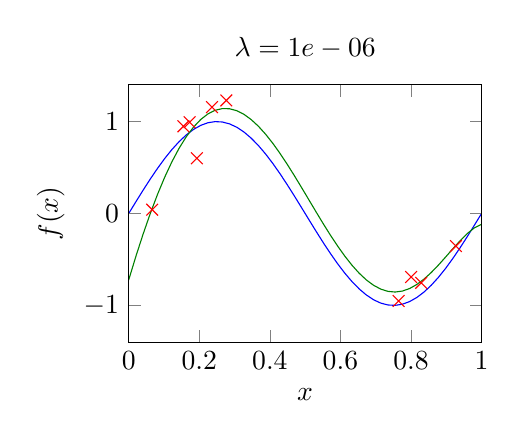
\begin{tikzpicture}

\begin{axis}[
title={$\lambda =1e-06$},
xlabel={$x$},
ylabel={$f(x)$},
xmin=0, xmax=1,
ymin=-1.4, ymax=1.4,
axis on top,
width=0.5\textwidth,
height=0.4\textwidth
]
\addplot [red, mark=x, mark size=3, only marks]
coordinates {
(0.236048089737435,1.15627363601475)
(0.15497227080241,0.948250349180675)
(0.0665150956795899,0.0414178360950077)
(0.800452351495809,-0.690913425000795)
(0.765162602505438,-0.951934188124491)
(0.27668264344145,1.23021694041087)
(0.172664529285369,0.993397777097462)
(0.92747563142806,-0.354104773238093)
(0.828920048778419,-0.754422446814427)
(0.19343561801924,0.600940658157845)

};
\addplot [blue]
coordinates {
(0,0)
(0.0204081632653061,0.127877161684506)
(0.0408163265306122,0.253654583909507)
(0.0612244897959184,0.375267004879374)
(0.0816326530612245,0.490717552003938)
(0.102040816326531,0.598110530491216)
(0.122448979591837,0.695682550603486)
(0.142857142857143,0.78183148246803)
(0.163265306122449,0.855142763005346)
(0.183673469387755,0.914412623015812)
(0.204081632653061,0.95866785303666)
(0.224489795918367,0.98718178341445)
(0.244897959183673,0.999486216200688)
(0.26530612244898,0.995379112949198)
(0.285714285714286,0.974927912181824)
(0.306122448979592,0.93846842204976)
(0.326530612244898,0.886599306373)
(0.346938775510204,0.820172254596956)
(0.36734693877551,0.740277997075316)
(0.387755102040816,0.648228395307788)
(0.408163265306122,0.545534901210549)
(0.428571428571429,0.433883739117558)
(0.448979591836735,0.315108218023621)
(0.469387755102041,0.191158628701373)
(0.489795918367347,0.0640702199807132)
(0.510204081632653,-0.064070219980713)
(0.530612244897959,-0.191158628701372)
(0.551020408163265,-0.31510821802362)
(0.571428571428571,-0.433883739117558)
(0.591836734693878,-0.545534901210548)
(0.612244897959184,-0.648228395307788)
(0.63265306122449,-0.740277997075315)
(0.653061224489796,-0.820172254596956)
(0.673469387755102,-0.886599306373)
(0.693877551020408,-0.93846842204976)
(0.714285714285714,-0.974927912181823)
(0.73469387755102,-0.995379112949198)
(0.755102040816326,-0.999486216200688)
(0.775510204081633,-0.98718178341445)
(0.795918367346939,-0.958667853036661)
(0.816326530612245,-0.914412623015813)
(0.836734693877551,-0.855142763005346)
(0.857142857142857,-0.78183148246803)
(0.877551020408163,-0.695682550603487)
(0.897959183673469,-0.598110530491217)
(0.918367346938775,-0.490717552003939)
(0.938775510204082,-0.375267004879375)
(0.959183673469388,-0.253654583909507)
(0.979591836734694,-0.127877161684507)
(1,-2.44929359829471e-16)

};
\addplot [green!50.0!black]
coordinates {
(0,-0.7225904673913)
(0.0204081632653061,-0.465634436482003)
(0.0408163265306122,-0.224081204019446)
(0.0612244897959184,0.000697422514947122)
(0.0816326530612245,0.207473023684331)
(0.102040816326531,0.395174346421548)
(0.122448979591837,0.562899276545063)
(0.142857142857143,0.709925005465732)
(0.163265306122449,0.8357163910844)
(0.183673469387755,0.939932512880322)
(0.204081632653061,1.02243142119041)
(0.224489795918367,1.08327308067934)
(0.244897959183673,1.12272050800041)
(0.26530612244898,1.14123910364735)
(0.285714285714286,1.13949417799681)
(0.306122448979592,1.11834667154184)
(0.326530612244898,1.07884706931603)
(0.346938775510204,1.02222750950864)
(0.36734693877551,0.949892086270419)
(0.387755102040816,0.863405346710369)
(0.408163265306122,0.764478982083247)
(0.428571428571429,0.654956713167947)
(0.448979591836735,0.5367973698367)
(0.469387755102041,0.412056164815093)
(0.489795918367347,0.282864161632927)
(0.510204081632653,0.151405936765901)
(0.530612244897959,0.0198954359681234)
(0.551020408163265,-0.109449975204554)
(0.571428571428571,-0.234437266680357)
(0.591836734693878,-0.352927304966593)
(0.612244897959184,-0.462866220053835)
(0.63265306122449,-0.562318578129254)
(0.653061224489796,-0.649502360099137)
(0.673469387755102,-0.722825745920579)
(0.693877551020408,-0.780925704742339)
(0.714285714285714,-0.822708390854878)
(0.73469387755102,-0.847391345449538)
(0.755102040816326,-0.854547504186941)
(0.775510204081633,-0.844151010574521)
(0.795918367346939,-0.816624835153229)
(0.816326530612245,-0.772890200493442)
(0.836734693877551,-0.714417812000009)
(0.857142857142857,-0.643280894526462)
(0.877551020408163,-0.562210034798449)
(0.897959183673469,-0.474649829646314)
(0.918367346938775,-0.384817340046766)
(0.938775510204082,-0.297762350973873)
(0.959183673469388,-0.21942943705913)
(0.979591836734694,-0.156721834060683)
(1,-0.117567116141792)

};
\path [draw=black, fill opacity=0] (axis cs:13,1.4)--(axis cs:13,1.4);

\path [draw=black, fill opacity=0] (axis cs:1,13)--(axis cs:1,13);

\path [draw=black, fill opacity=0] (axis cs:13,-1.4)--(axis cs:13,-1.4);

\path [draw=black, fill opacity=0] (axis cs:0,13)--(axis cs:0,13);

\end{axis}

\end{tikzpicture}\hfill{}% This file was created by matplotlib v0.1.0.
% Copyright (c) 2010--2014, Nico Schlömer <nico.schloemer@gmail.com>
% All rights reserved.
% 
% The lastest updates can be retrieved from
% 
% https://github.com/nschloe/matplotlib2tikz
% 
% where you can also submit bug reports and leavecomments.
% 
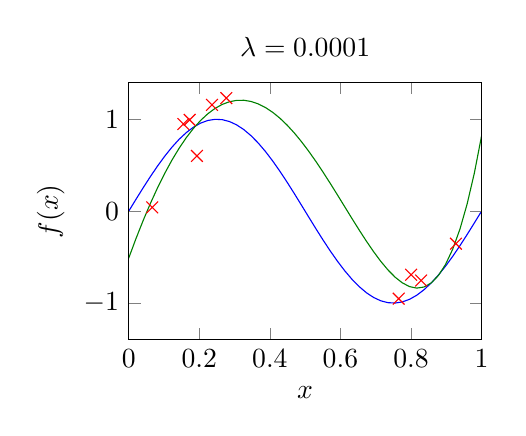
\begin{tikzpicture}

\begin{axis}[
title={$\lambda =0.0001$},
xlabel={$x$},
ylabel={$f(x)$},
xmin=0, xmax=1,
ymin=-1.4, ymax=1.4,
axis on top,
width=0.5\textwidth,
height=0.4\textwidth
]
\addplot [red, mark=x, mark size=3, only marks]
coordinates {
(0.236048089737435,1.15627363601475)
(0.15497227080241,0.948250349180675)
(0.0665150956795899,0.0414178360950077)
(0.800452351495809,-0.690913425000795)
(0.765162602505438,-0.951934188124491)
(0.27668264344145,1.23021694041087)
(0.172664529285369,0.993397777097462)
(0.92747563142806,-0.354104773238093)
(0.828920048778419,-0.754422446814427)
(0.19343561801924,0.600940658157845)

};
\addplot [blue]
coordinates {
(0,0)
(0.0204081632653061,0.127877161684506)
(0.0408163265306122,0.253654583909507)
(0.0612244897959184,0.375267004879374)
(0.0816326530612245,0.490717552003938)
(0.102040816326531,0.598110530491216)
(0.122448979591837,0.695682550603486)
(0.142857142857143,0.78183148246803)
(0.163265306122449,0.855142763005346)
(0.183673469387755,0.914412623015812)
(0.204081632653061,0.95866785303666)
(0.224489795918367,0.98718178341445)
(0.244897959183673,0.999486216200688)
(0.26530612244898,0.995379112949198)
(0.285714285714286,0.974927912181824)
(0.306122448979592,0.93846842204976)
(0.326530612244898,0.886599306373)
(0.346938775510204,0.820172254596956)
(0.36734693877551,0.740277997075316)
(0.387755102040816,0.648228395307788)
(0.408163265306122,0.545534901210549)
(0.428571428571429,0.433883739117558)
(0.448979591836735,0.315108218023621)
(0.469387755102041,0.191158628701373)
(0.489795918367347,0.0640702199807132)
(0.510204081632653,-0.064070219980713)
(0.530612244897959,-0.191158628701372)
(0.551020408163265,-0.31510821802362)
(0.571428571428571,-0.433883739117558)
(0.591836734693878,-0.545534901210548)
(0.612244897959184,-0.648228395307788)
(0.63265306122449,-0.740277997075315)
(0.653061224489796,-0.820172254596956)
(0.673469387755102,-0.886599306373)
(0.693877551020408,-0.93846842204976)
(0.714285714285714,-0.974927912181823)
(0.73469387755102,-0.995379112949198)
(0.755102040816326,-0.999486216200688)
(0.775510204081633,-0.98718178341445)
(0.795918367346939,-0.958667853036661)
(0.816326530612245,-0.914412623015813)
(0.836734693877551,-0.855142763005346)
(0.857142857142857,-0.78183148246803)
(0.877551020408163,-0.695682550603487)
(0.897959183673469,-0.598110530491217)
(0.918367346938775,-0.490717552003939)
(0.938775510204082,-0.375267004879375)
(0.959183673469388,-0.253654583909507)
(0.979591836734694,-0.127877161684507)
(1,-2.44929359829471e-16)

};
\addplot [green!50.0!black]
coordinates {
(0,-0.51080427506794)
(0.0204081632653061,-0.300241019104784)
(0.0408163265306122,-0.102497794996123)
(0.0612244897959184,0.0821434033526013)
(0.0816326530612245,0.253417580013832)
(0.102040816326531,0.411079523757286)
(0.122448979591837,0.554906764088884)
(0.142857142857143,0.684702696609222)
(0.163265306122449,0.800299877691577)
(0.183673469387755,0.901563488479453)
(0.204081632653061,0.988394968203666)
(0.224489795918367,1.06073581681896)
(0.244897959183673,1.11857156696019)
(0.26530612244898,1.16193592521799)
(0.285714285714286,1.19091508273402)
(0.306122448979592,1.20565219511576)
(0.326530612244898,1.20635203167082)
(0.346938775510204,1.19328579396075)
(0.36734693877551,1.16679610367451)
(0.387755102040816,1.12730215982131)
(0.408163265306122,1.07530506524315)
(0.428571428571429,1.0113933224468)
(0.448979591836735,0.93624849875532)
(0.469387755102041,0.850651060779187)
(0.489795918367347,0.755486378206884)
(0.510204081632653,0.651750896915072)
(0.530612244897959,0.540558481398286)
(0.551020408163265,0.423146926518167)
(0.571428571428571,0.300884638572248)
(0.591836734693878,0.175277485682251)
(0.612244897959184,0.0479758175019536)
(0.63265306122449,-0.0792183457554324)
(0.653061224489796,-0.204343954970329)
(0.673469387755102,-0.325273404450326)
(0.693877551020408,-0.439704834944173)
(0.714285714285714,-0.545154267336243)
(0.73469387755102,-0.638947567021445)
(0.755102040816326,-0.718212238960607)
(0.775510204081633,-0.779869053416321)
(0.795918367346939,-0.820623502369237)
(0.816326530612245,-0.836957086614839)
(0.836734693877551,-0.825118433540664)
(0.857142857142857,-0.781114245583996)
(0.877551020408163,-0.700700079370009)
(0.897959183673469,-0.579370955530394)
(0.918367346938775,-0.412351799202406)
(0.938775510204082,-0.194587711208429)
(0.959183673469388,0.0792659300840506)
(0.979591836734694,0.414853536221978)
(1,0.818129545445799)

};
\path [draw=black, fill opacity=0] (axis cs:13,1.4)--(axis cs:13,1.4);

\path [draw=black, fill opacity=0] (axis cs:1,13)--(axis cs:1,13);

\path [draw=black, fill opacity=0] (axis cs:13,-1.4)--(axis cs:13,-1.4);

\path [draw=black, fill opacity=0] (axis cs:0,13)--(axis cs:0,13);

\end{axis}

\end{tikzpicture}% This file was created by matplotlib v0.1.0.
% Copyright (c) 2010--2014, Nico Schlömer <nico.schloemer@gmail.com>
% All rights reserved.
% 
% The lastest updates can be retrieved from
% 
% https://github.com/nschloe/matplotlib2tikz
% 
% where you can also submit bug reports and leavecomments.
% 
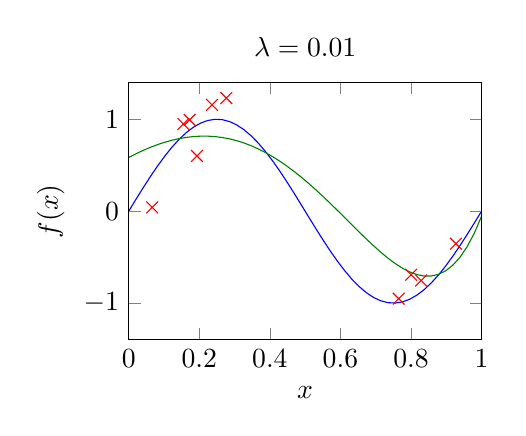
\begin{tikzpicture}

\begin{axis}[
title={$\lambda =0.01$},
xlabel={$x$},
ylabel={$f(x)$},
xmin=0, xmax=1,
ymin=-1.4, ymax=1.4,
axis on top,
width=0.5\textwidth,
height=0.4\textwidth
]
\addplot [red, mark=x, mark size=3, only marks]
coordinates {
(0.236048089737435,1.15627363601475)
(0.15497227080241,0.948250349180675)
(0.0665150956795899,0.0414178360950077)
(0.800452351495809,-0.690913425000795)
(0.765162602505438,-0.951934188124491)
(0.27668264344145,1.23021694041087)
(0.172664529285369,0.993397777097462)
(0.92747563142806,-0.354104773238093)
(0.828920048778419,-0.754422446814427)
(0.19343561801924,0.600940658157845)

};
\addplot [blue]
coordinates {
(0,0)
(0.0204081632653061,0.127877161684506)
(0.0408163265306122,0.253654583909507)
(0.0612244897959184,0.375267004879374)
(0.0816326530612245,0.490717552003938)
(0.102040816326531,0.598110530491216)
(0.122448979591837,0.695682550603486)
(0.142857142857143,0.78183148246803)
(0.163265306122449,0.855142763005346)
(0.183673469387755,0.914412623015812)
(0.204081632653061,0.95866785303666)
(0.224489795918367,0.98718178341445)
(0.244897959183673,0.999486216200688)
(0.26530612244898,0.995379112949198)
(0.285714285714286,0.974927912181824)
(0.306122448979592,0.93846842204976)
(0.326530612244898,0.886599306373)
(0.346938775510204,0.820172254596956)
(0.36734693877551,0.740277997075316)
(0.387755102040816,0.648228395307788)
(0.408163265306122,0.545534901210549)
(0.428571428571429,0.433883739117558)
(0.448979591836735,0.315108218023621)
(0.469387755102041,0.191158628701373)
(0.489795918367347,0.0640702199807132)
(0.510204081632653,-0.064070219980713)
(0.530612244897959,-0.191158628701372)
(0.551020408163265,-0.31510821802362)
(0.571428571428571,-0.433883739117558)
(0.591836734693878,-0.545534901210548)
(0.612244897959184,-0.648228395307788)
(0.63265306122449,-0.740277997075315)
(0.653061224489796,-0.820172254596956)
(0.673469387755102,-0.886599306373)
(0.693877551020408,-0.93846842204976)
(0.714285714285714,-0.974927912181823)
(0.73469387755102,-0.995379112949198)
(0.755102040816326,-0.999486216200688)
(0.775510204081633,-0.98718178341445)
(0.795918367346939,-0.958667853036661)
(0.816326530612245,-0.914412623015813)
(0.836734693877551,-0.855142763005346)
(0.857142857142857,-0.78183148246803)
(0.877551020408163,-0.695682550603487)
(0.897959183673469,-0.598110530491217)
(0.918367346938775,-0.490717552003939)
(0.938775510204082,-0.375267004879375)
(0.959183673469388,-0.253654583909507)
(0.979591836734694,-0.127877161684507)
(1,-2.44929359829471e-16)

};
\addplot [green!50.0!black]
coordinates {
(0,0.584185425330399)
(0.0204081632653061,0.624348353392445)
(0.0408163265306122,0.661155901138946)
(0.0612244897959184,0.694453409940694)
(0.0816326530612245,0.7240853455842)
(0.102040816326531,0.749896372372221)
(0.122448979591837,0.771732593515947)
(0.142857142857143,0.78944295781885)
(0.163265306122449,0.802880832652196)
(0.183673469387755,0.811905743222209)
(0.204081632653061,0.816385278128904)
(0.224489795918367,0.81619716121658)
(0.244897959183673,0.811231489715961)
(0.26530612244898,0.801393138678017)
(0.285714285714286,0.786604331699429)
(0.306122448979592,0.766807377939719)
(0.326530612244898,0.741967575430047)
(0.346938775510204,0.712076280673659)
(0.36734693877551,0.677154144537999)
(0.387755102040816,0.637254514438486)
(0.408163265306122,0.592467002813939)
(0.428571428571429,0.542921221893677)
(0.448979591836735,0.48879068475627)
(0.469387755102041,0.430296872679952)
(0.489795918367347,0.367713468784698)
(0.510204081632653,0.301370757965954)
(0.530612244897959,0.231660193120037)
(0.551020408163265,0.159039127661183)
(0.571428571428571,0.0840357143302718)
(0.591836734693878,0.00725397029519409)
(0.612244897959184,-0.0706209914571067)
(0.63265306122449,-0.148817564436942)
(0.653061224489796,-0.226472084676519)
(0.673469387755102,-0.302623100462925)
(0.693877551020408,-0.376205475779447)
(0.714285714285714,-0.446044327455238)
(0.73469387755102,-0.510848796023319)
(0.755102040816326,-0.569205650286917)
(0.775510204081633,-0.619572725594149)
(0.795918367346939,-0.660272195821042)
(0.816326530612245,-0.689483679062897)
(0.836734693877551,-0.705237177033983)
(0.857142857142857,-0.705405848175584)
(0.877551020408163,-0.687698614472373)
(0.897959183673469,-0.649652601977137)
(0.918367346938775,-0.58862541504383)
(0.938775510204082,-0.501787244268978)
(0.959183673469388,-0.386112808141413)
(0.979591836734694,-0.23837312840035)
(1,-0.0551271391018138)

};
\path [draw=black, fill opacity=0] (axis cs:13,1.4)--(axis cs:13,1.4);

\path [draw=black, fill opacity=0] (axis cs:1,13)--(axis cs:1,13);

\path [draw=black, fill opacity=0] (axis cs:13,-1.4)--(axis cs:13,-1.4);

\path [draw=black, fill opacity=0] (axis cs:0,13)--(axis cs:0,13);

\end{axis}

\end{tikzpicture}\hfill{}% This file was created by matplotlib v0.1.0.
% Copyright (c) 2010--2014, Nico Schlömer <nico.schloemer@gmail.com>
% All rights reserved.
% 
% The lastest updates can be retrieved from
% 
% https://github.com/nschloe/matplotlib2tikz
% 
% where you can also submit bug reports and leavecomments.
% 
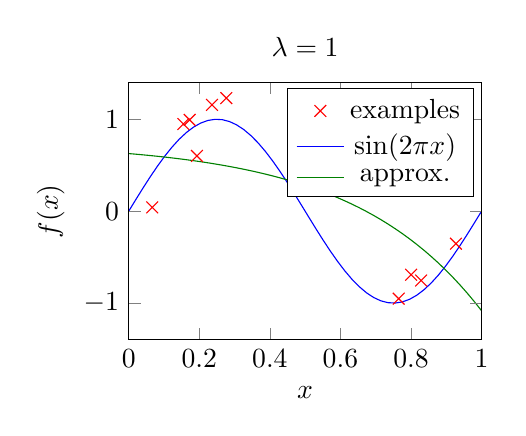
\begin{tikzpicture}

\begin{axis}[
title={$\lambda =1$},
xlabel={$x$},
ylabel={$f(x)$},
xmin=0, xmax=1,
ymin=-1.4, ymax=1.4,
axis on top,
width=0.5\textwidth,
height=0.4\textwidth,
legend entries={{examples},{$\sin(2\pi x)$},{approx.}}
]
\addplot [red, mark=x, mark size=3, only marks]
coordinates {
(0.236048089737435,1.15627363601475)
(0.15497227080241,0.948250349180675)
(0.0665150956795899,0.0414178360950077)
(0.800452351495809,-0.690913425000795)
(0.765162602505438,-0.951934188124491)
(0.27668264344145,1.23021694041087)
(0.172664529285369,0.993397777097462)
(0.92747563142806,-0.354104773238093)
(0.828920048778419,-0.754422446814427)
(0.19343561801924,0.600940658157845)

};
\addplot [blue]
coordinates {
(0,0)
(0.0204081632653061,0.127877161684506)
(0.0408163265306122,0.253654583909507)
(0.0612244897959184,0.375267004879374)
(0.0816326530612245,0.490717552003938)
(0.102040816326531,0.598110530491216)
(0.122448979591837,0.695682550603486)
(0.142857142857143,0.78183148246803)
(0.163265306122449,0.855142763005346)
(0.183673469387755,0.914412623015812)
(0.204081632653061,0.95866785303666)
(0.224489795918367,0.98718178341445)
(0.244897959183673,0.999486216200688)
(0.26530612244898,0.995379112949198)
(0.285714285714286,0.974927912181824)
(0.306122448979592,0.93846842204976)
(0.326530612244898,0.886599306373)
(0.346938775510204,0.820172254596956)
(0.36734693877551,0.740277997075316)
(0.387755102040816,0.648228395307788)
(0.408163265306122,0.545534901210549)
(0.428571428571429,0.433883739117558)
(0.448979591836735,0.315108218023621)
(0.469387755102041,0.191158628701373)
(0.489795918367347,0.0640702199807132)
(0.510204081632653,-0.064070219980713)
(0.530612244897959,-0.191158628701372)
(0.551020408163265,-0.31510821802362)
(0.571428571428571,-0.433883739117558)
(0.591836734693878,-0.545534901210548)
(0.612244897959184,-0.648228395307788)
(0.63265306122449,-0.740277997075315)
(0.653061224489796,-0.820172254596956)
(0.673469387755102,-0.886599306373)
(0.693877551020408,-0.93846842204976)
(0.714285714285714,-0.974927912181823)
(0.73469387755102,-0.995379112949198)
(0.755102040816326,-0.999486216200688)
(0.775510204081633,-0.98718178341445)
(0.795918367346939,-0.958667853036661)
(0.816326530612245,-0.914412623015813)
(0.836734693877551,-0.855142763005346)
(0.857142857142857,-0.78183148246803)
(0.877551020408163,-0.695682550603487)
(0.897959183673469,-0.598110530491217)
(0.918367346938775,-0.490717552003939)
(0.938775510204082,-0.375267004879375)
(0.959183673469388,-0.253654583909507)
(0.979591836734694,-0.127877161684507)
(1,-2.44929359829471e-16)

};
\addplot [green!50.0!black]
coordinates {
(0,0.626740504601331)
(0.0204081632653061,0.619964124133218)
(0.0408163265306122,0.612787706947775)
(0.0612244897959184,0.605190267463991)
(0.0816326530612245,0.597149531789616)
(0.102040816326531,0.588641848223021)
(0.122448979591837,0.579642092249008)
(0.142857142857143,0.570123566028575)
(0.163265306122449,0.560057892382633)
(0.183673469387755,0.549414903269679)
(0.204081632653061,0.538162522757418)
(0.224489795918367,0.526266644488345)
(0.244897959183673,0.513691003639273)
(0.26530612244898,0.500397043374821)
(0.285714285714286,0.486343775794851)
(0.306122448979592,0.471487637375863)
(0.326530612244898,0.455782338906336)
(0.346938775510204,0.439178709916032)
(0.36734693877551,0.421624537599248)
(0.387755102040816,0.403064400232019)
(0.408163265306122,0.38343949508328)
(0.428571428571429,0.362687460819982)
(0.448979591836735,0.340742194406151)
(0.469387755102041,0.317533662495917)
(0.489795918367347,0.292987707320481)
(0.510204081632653,0.267025847069047)
(0.530612244897959,0.2395650707637)
(0.551020408163265,0.210517627628239)
(0.571428571428571,0.179790810950967)
(0.591836734693878,0.147286736441433)
(0.612244897959184,0.112902115081123)
(0.63265306122449,0.0765280204681117)
(0.653061224489796,0.0380496506556607)
(0.673469387755102,-0.00265391551522297)
(0.693877551020408,-0.0457099675892805)
(0.714285714285714,-0.0912524181765384)
(0.73469387755102,-0.139422063137894)
(0.755102040816326,-0.190366847276744)
(0.775510204081633,-0.244242135536665)
(0.795918367346939,-0.301210989705135)
(0.816326530612245,-0.361444450623306)
(0.836734693877551,-0.425121825901818)
(0.857142857142857,-0.492430983142667)
(0.877551020408163,-0.563568648667109)
(0.897959183673469,-0.638740711749623)
(0.918367346938775,-0.718162534357909)
(0.938775510204082,-0.802059266398941)
(0.959183673469388,-0.890666166471061)
(0.979591836734694,-0.984228928122121)
(1,-1.08300401161367)

};
\path [draw=black, fill opacity=0] (axis cs:13,1.4)--(axis cs:13,1.4);

\path [draw=black, fill opacity=0] (axis cs:1,13)--(axis cs:1,13);

\path [draw=black, fill opacity=0] (axis cs:13,-1.4)--(axis cs:13,-1.4);

\path [draw=black, fill opacity=0] (axis cs:0,13)--(axis cs:0,13);

\end{axis}

\end{tikzpicture}\caption{Results of ridge regression for $\lambda\in\left\{ 0,10^{-8},10^{-6},10^{-4},10^{-2},1\right\} $\label{fig:ridge-regression}}
\end{figure}
